\documentclass[12pt]{article}
\usepackage{times}
\usepackage{geometry}
\usepackage[english]{babel}
\usepackage[utf8]{inputenc}
\usepackage{fancyhdr}
\usepackage{graphicx}
\usepackage{titlesec}
\usepackage{minted}
\usepackage{lipsum}  % Include lipsum package for dummy text

\setlength{\headheight}{15.2pt}
\setcounter{secnumdepth}{4}

\titleformat{\paragraph}
{\normalfont\normalsize\bfseries}{\theparagraph}{1em}{}
\titlespacing*{\paragraph}
{0pt}{3.25ex plus 1ex minus .2ex}{1.5ex plus .2ex}

\rfoot{Pg: \thepage}

\geometry{
   a4paper,
   left = 20mm,
   top = 20mm,
}

\begin{document}
\thispagestyle{empty}

\section*{}
{\LARGE\makebox[\textwidth]{\textbf{KATHMANDU UNIVERSITY}}}

\centerline{Department of Computer Science and Engineering}
\centerline{Dhulikhel, Kavre}
\begin{figure}[h]
    \centerline{
\includegraphics[width=50.546mm,height=50.546mm]{KU_Logo.png}}
\end{figure}

\centerline{\textbf{An Assignment Report}}
\centerline{on}
\centerline{\underline{\textbf{"Exploration of Search Methods for various AI search space Problems"}}}
\vspace*{5mm}
\centerline{\textbf{Missionaries and Cannibals Problem}}
\centerline{\textbf{8 Puzzle Problem}}
\centerline{\textbf{Water Jug Problem}}

\vspace*{8mm}

\centerline{\textbf{[Code No. : COMP 472]}}
\centerline{(For partial fulfillment of 4th Year/ 7th Semester in Computer Science)}

\vspace*{15mm}

\centerline{\textbf{Submitted by}}
\centerline{\textbf{Abha Acharya (Roll No. 1)}}
\centerline{\textbf{Aayush Pokharel (Roll No. 43)}}

\vspace*{16mm}

\centerline{\underline{\textbf{Submitted to}}}
\centerline{\textbf{Santosh Khanal}}
\centerline{\textbf{Assistant Professor}}
\centerline{\textbf{Dept of Computer Science and Engineering}}
\vspace*{30mm}

\centerline{\textbf{Submission Date: 4th January, 2024}}

\clearpage

\section*{Abstract}
\thispagestyle{empty}
This report delves into the exploration of search methods through the analysis and solution of three distinct problems: the Missionaries and Cannibals Problem, the 8 Puzzle Problem, and the Water Jug Problem. Each problem is systematically defined, and their respective search space representations are elucidated. The report presents solutions employing Depth-First Search (DFS), Breadth-First Search (BFS) and A* Search for the problem, shedding light on the intricacies of the algorithms' application.

The Missionaries and Cannibals Problem, requiring the transportation of missionaries and cannibals across a river while adhering to specific constraints, is tackled through DFS and BFS approaches. The 8 Puzzle Problem, a classic sliding puzzle, and the Water Jug Problem, involving the strategic manipulation of water volumes to achieve a target, are also explored using DFS and BFS strategies where as the 8 Sliding Puzzle Problem is tacked with A* and BFS approaches.

The report culminates in an examination of the technologies and libraries instrumental in the implementation of the search algorithms. The insights gained from the solutions highlight the efficacy of search methods in addressing complex problems across diverse domains. The report concludes with suggestions for further work, emphasizing the potential for enhanced heuristics, parallelization, real-world applications, and improved user interaction to augment the capabilities and applicability of search methods in future endeavors.




\clearpage
\thispagestyle{empty}
\tableofcontents

\clearpage
\thispagestyle{empty}
\listoffigures
\clearpage

\pagenumbering{arabic}
\section{Introduction}
\subsection{Background}

Artificial Intelligence (AI) stands as a transformative force across diverse domains, reshaping the landscape of machine 
perception, reasoning, and decision-making. Central to numerous AI applications are search methods, sophisticated 
algorithms meticulously crafted to traverse expansive solution spaces and unearth optimal or satisfactory solutions. 
These methodologies form the bedrock of AI, playing a pivotal role in problem-solving, decision-making, and optimization. 
This overview aims to succinctly underscore the profound significance of search methods and their multifaceted applications 
within the realm of AI.

% \subsection{Significance of Search Methods}

% In the intricate realm of complex problem-solving, where real-world challenges exhibit layers of complexity, uncertainty, 
% and myriad potential solutions, search methods emerge as beacons of efficiency. These algorithms introduce a systematic 
% approach to navigate through solution spaces, providing a crucial toolset for addressing intricate problems with unparalleled 
% effectiveness.


% The breadth of applications for search methods is vast and impactful. In decision-making processes, where the evaluation of 
% multiple alternatives involves nuanced trade-offs, search algorithms step in as facilitators. By exploring decision trees or 
% state spaces, they empower intelligent systems to make informed choices based on predefined criteria, offering clarity in the 
% face of complexity.


% In the realm of optimization and resource management, search methods shine as valuable assets. Their contribution extends to 
% identifying optimal solutions, be it minimizing or maximizing objective functions, or strategically optimizing the allocation 
% of resources. This versatility equips AI systems to navigate challenges ranging from resource scarcity to complex optimization 
% scenarios.


% Games and strategic scenarios, demanding optimal moves and planning, find a fundamental ally in search algorithms such as 
% minimax. These algorithms underpin the development of intelligent agents for game playing, enhancing strategic decision-making 
% and introducing a layer of sophistication to AI's gaming capabilities.

% In the domain of Natural Language Processing (NLP) and information retrieval, search algorithms play a vital role. They tackle 
% the challenge of extracting pertinent information from extensive datasets or documents, enhancing the overall performance of NLP 
% applications.

% For autonomous systems tasked with navigating intricate environments in real-time, search methods emerge as indispensable. 
% Particularly in path planning, these algorithms facilitate seamless navigation for robots and autonomous agents, enabling them 
% to negotiate complex terrains while avoiding obstacles.

% In summary, search methods stand as the cornerstone of diverse AI applications, offering systematic and efficient approaches 
% to unravel complex problems. Their adaptability and versatility position them as indispensable tools, enabling the development 
% of intelligent systems capable of navigating, learning, and decision-making in a myriad of dynamic environments.

\subsection{Significance of Search Methods}

In the intricate realm of complex problem-solving, where real-world challenges exhibit layers of complexity, uncertainty, 
and myriad potential solutions, search methods emerge as beacons of efficiency~\cite{russell2009ai}. These algorithms introduce a systematic 
approach to navigate through solution spaces, providing a crucial toolset for addressing intricate problems with unparalleled 
effectiveness.

The breadth of applications for search methods is vast and impactful. In decision-making processes, where the evaluation of 
multiple alternatives involves nuanced trade-offs, search algorithms step in as facilitators~\cite{nilsson2014principles}. By exploring decision trees or 
state spaces, they empower intelligent systems to make informed choices based on predefined criteria, offering clarity in the 
face of complexity.

In the realm of optimization and resource management, search methods shine as valuable assets~\cite{cormen2009introduction}. Their contribution extends to 
identifying optimal solutions, be it minimizing or maximizing objective functions, or strategically optimizing the allocation 
of resources. This versatility equips AI systems to navigate challenges ranging from resource scarcity to complex optimization 
scenarios.

Games and strategic scenarios, demanding optimal moves and planning, find a fundamental ally in search algorithms such as 
minimax~\cite{russell2009ai}. These algorithms underpin the development of intelligent agents for game playing, enhancing strategic decision-making 
and introducing a layer of sophistication to AI's gaming capabilities.

In the domain of Natural Language Processing (NLP) and information retrieval, search algorithms play a vital role~\cite{cormen2009introduction}. They tackle 
the challenge of extracting pertinent information from extensive datasets or documents, enhancing the overall performance of NLP 
applications.

For autonomous systems tasked with navigating intricate environments in real-time, search methods emerge as indispensable. 
Particularly in path planning, these algorithms facilitate seamless navigation for robots and autonomous agents, enabling them 
to negotiate complex terrains while avoiding obstacles~\cite{poole1998computational}.

In summary, search methods stand as the cornerstone of diverse AI applications, offering systematic and efficient approaches 
to unraveling complex problems. Their adaptability and versatility position them as indispensable tools, enabling the development 
of intelligent systems capable of navigating, learning, and decision-making in a myriad of dynamic environments.


\subsection{Objective}

The objectives of this assignment are; 
\begin{itemize}
    \item to explore search methods for various AI problems,
    \item to analyze the performance of search algorithms in different scenarios,
    \item to evaluate the effectiveness of search methods in problem-solving and decision-making,
    \item to synthesize insights for effective application of search methods in diverse problem-solving scenarios within Artificial Intelligence.
    \item gain practical experience in applying search methods to solve real-world problems.
\end{itemize}

\section{Missionaries and Cannibals Problem}
\subsection{Problem Definition}
The Missionaries and Cannibals Problem is a classic puzzle or game representing a river-crossing scenario involving missionaries, 
cannibals, and a boat. The puzzle typically features three missionaries and three cannibals on one side of a river along with a 
boat that can carry a maximum of two individuals. The objective is to transport all individuals from one side of the river 
to the other without violating specific constraints.
\\\\
\textbf{The constraints are as follows:}
    \begin{itemize}
        \item The boat can carry a maximum of two individuals.
        \item The boat cannot cross the river without any passengers.
        \item The cannibals cannot outnumber the missionaries on either side of the river.
    \end{itemize}
The challenge is to devise a sequence of boat trips that adheres to these constraints, ultimately moving all missionaries and cannibals to the opposite side of the river without any harm befalling the missionaries.

\subsection{Search Space Representation}
To represent the search space for the Missionaries and Cannibals Problem, the code utilizes a Python class named \texttt{Solution}. 
The key components of the search space representation are outlined below:
\begin{minted}[breaklines]{python}
    class Solution():
        def __init__(self):
            # Initial state with 3 missionaries, 3 cannibals, and the boat on the right side
            self.start_state = (3, 3, 1)
            
            # Goal state with 0 missionaries, 0 cannibals, and the boat on the left side
            self.goal_state = (0, 0, 0)
            
            # Possible movement options for the boat, represented as tuples (m, c)
            self.options = [(1, 0), (0, 1), (1, 1), (0, 2), (2, 0)]
            
            # Possible sides of the river where the boat can be
            self.boat_side = ["right", "left"]
            
            # Graph representation for visualization (using pydot.Dot)
            self.graph = pydot.Dot(graph_type='graph', bgcolor="#ffffff", fontcolor="black", fontsize="24")      
            
            # Dictionary to keep track of visited states
            self.visited = {}
            
            # Flag to indicate if the problem has been solved
            self.solved = False
    \end{minted}
    \vspace*{5mm}
In this representation, the initial state (\texttt{start\_state}) is defined as having 3 missionaries, 3 cannibals, and the boat on the right side of the river. The goal state (\texttt{goal\_state}) is defined with 0 missionaries, 0 cannibals, and the boat on the left side. The \texttt{options} variable enumerates the possible movements of the boat, and \texttt{boat\_side} represents the two possible sides of the river where the boat can be.

The \texttt{graph} attribute is a pydot graph object, facilitating the visualization of the search space tree. The \texttt{visited} dictionary keeps track of the states that have been visited during the search process, and the \texttt{solved} flag indicates whether the problem has been successfully solved.

This comprehensive representation encapsulates the essential elements required for exploring the search space and finding a solution to the Missionaries and Cannibals Problem.

\clearpage
\subsection{Solution via DFS}
To explore the solution space using Depth-First Search (DFS), the algorithm systematically traverses the state space tree, prioritizing depth over breadth.
\\\\
\begin{figure}[h]
  \centerline{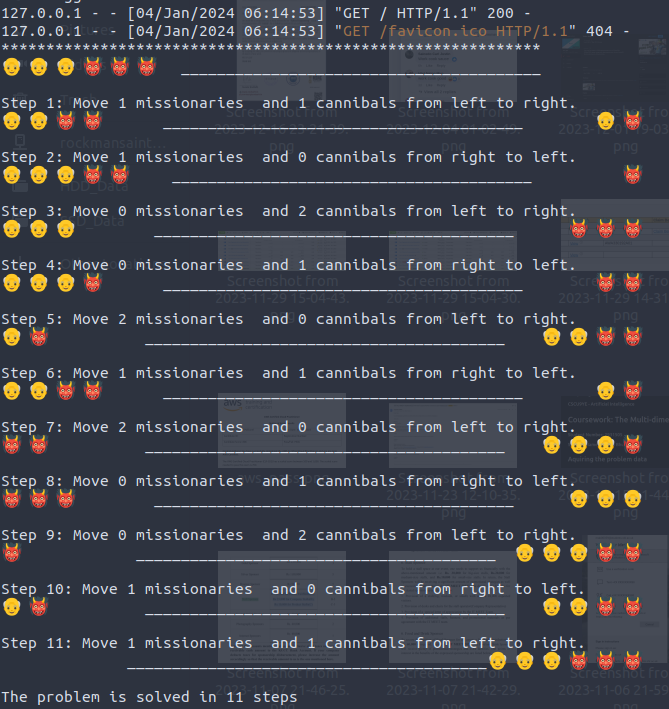
\includegraphics[width = 150mm]{MnC_DFS_demo.png}}
  \caption{Missionaries & Cannibals DFS Solution Demo}
  \label{fig}
\end{figure}
\clearpage
\begin{figure}[h]
  \centerline{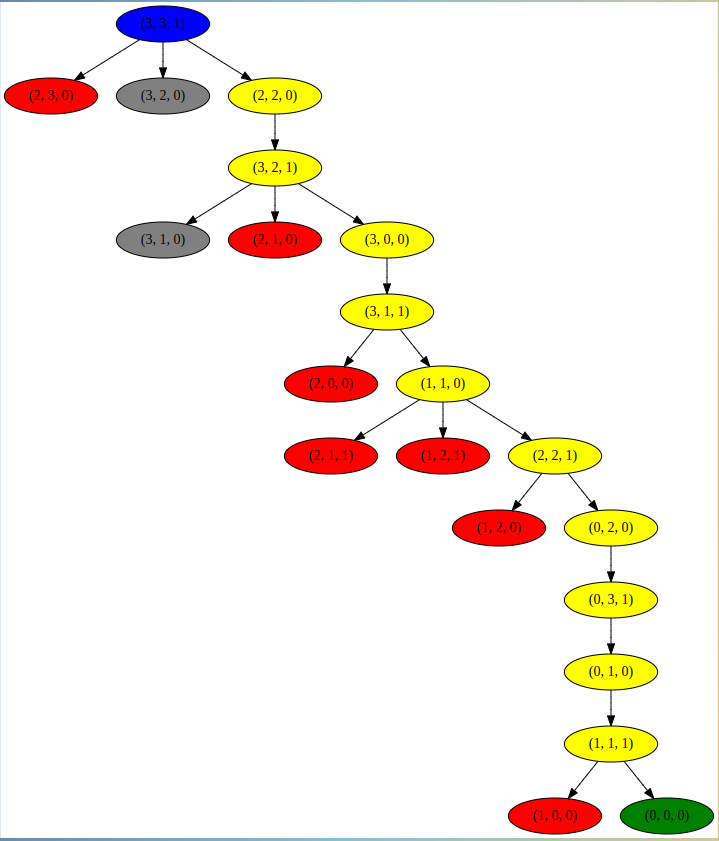
\includegraphics[width = 150mm]{MnC_DFS.png}}
  \caption{Missionaries & Cannibals DFS Solution Tree}
  \label{fig}
\end{figure}
\textbf{The relevant portions of the code for DFS are outlined below:}
\subsubsection*{Initialization and Base Cases}
\begin{minted}[breaklines]{python}
def dfs(self, number_missionaries, number_cannnibals, side, depth_level):
    # Mark the current state as visited
    self.visited[(number_missionaries, number_cannnibals, side)] = True
    
    # Draw the current state in the solution space tree
    u, v = self.draw_edge(number_missionaries, number_cannnibals, side, depth_level)
    
    # Base Cases for Start, Goal, and Cannibal Exceedance
    if self.is_start_state(number_missionaries, number_cannnibals, side):
        v.set_style("filled")
        v.set_fillcolor("blue")
    elif self.is_goal_state(number_missionaries, number_cannnibals, side):
        v.set_style("filled")
        v.set_fillcolor("green")
        return True
    elif self.number_of_cannibals_exceeds(number_missionaries, number_cannnibals):
        v.set_style("filled")
        v.set_fillcolor("red")
        return False
    else:
        v.set_style("filled")
        v.set_fillcolor("orange")
\end{minted}
    \vspace*{5mm}
In the beginning, the function initializes the state by marking it as visited and drawing the corresponding node in the solution space tree. It checks for base cases, such as whether the current state is the start state, goal state, or if the number of cannibals exceeds the number of missionaries on any side of the river.

\subsubsection*{Recursive Exploration}
\begin{minted}[breaklines]{python}
    solution_found = False
    operation = -1 if side == 1 else 1

    can_be_expanded = False

    for x, y in self.options:
        next_m, next_c, next_s = number_missionaries + operation * x, number_cannnibals + operation * y, int(not side)

        if (next_m, next_c, next_s) not in self.visited:
            if self.is_valid_move(next_m, next_c):
                can_be_expanded = True
                # Keep track of Parent state and corresponding move
                Parent[(next_m, next_c, next_s)] = (number_missionaries, number_cannnibals, side)
                Move[(next_m, next_c, next_s)] = (x, y, side)
                node_list[(next_m, next_c, next_s)] = v

                # Recursive call to explore the next state
                solution_found = (solution_found or self.dfs(next_m, next_c, next_s, depth_level + 1))
            
                if solution_found:
                    return True
\end{minted}
    \vspace*{5mm}
The function then enters a loop where it iterates through possible moves (carrying missionaries and cannibals in the boat) and recursively explores the resulting states. The recursion allows the algorithm to go deeper into the solution space until a solution is found or the exploration is exhausted.

\subsubsection*{Backtracking and Visualization}
\begin{minted}[breaklines]{python}
    if not can_be_expanded:
        v.set_style("filled")
        v.set_fillcolor("gray")

    self.solved = solution_found
    return solution_found
\end{minted}
    \vspace*{5mm}
If no further exploration is possible from the current state, the node in the solution space tree is marked as gray. The function then returns whether a solution was found or not.

Overall, the \texttt{dfs()} function implements a depth-first exploration strategy, where it explores as deeply as possible along each branch of the solution space before backtracking when necessary. The backtracking ensures that all possibilities are explored, leading to the discovery of a valid solution.

\clearpage
\subsection{Solution via BFS}
The \texttt{bfs()} function is responsible for performing Breadth-First Search (BFS) on the state space of the Missionaries and Cannibals Problem. 
\begin{figure}[h]
  \centerline{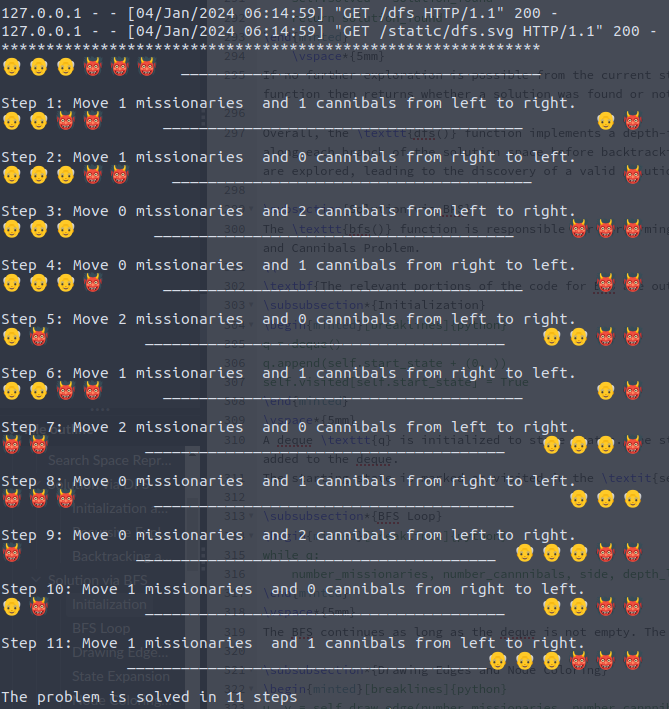
\includegraphics[width = 150mm]{MnC_BFS_demo.png}}
  \caption{Missionaries & Cannibals BFS Solution Demo}
  \label{fig}
\end{figure}

\\
\textbf{The relevant portions of the code for BFS are outlined below:}
\subsubsection*{Initialization}
\begin{minted}[breaklines]{python}
q = deque()
q.append(self.start_state + (0, ))
self.visited[self.start_state] = True
\end{minted}
\vspace*{5mm}
A deque \texttt{q} is initialized to store states. The starting state with an additional element \texttt{depth\_level} is added to the deque.
The starting state is marked as visited in the \textit{self. visited} dictionary.

\subsubsection*{BFS Loop}
\begin{minted}[breaklines]{python}
while q:
    number_missionaries, number_cannnibals, side, depth_level = q.popleft()
\end{minted}
\vspace*{5mm}
The BFS continues as long as the deque is not empty. The leftmost (oldest) state is dequeued, and its components are unpacked.

\subsubsection*{Drawing Edges and Node Coloring}
\begin{minted}[breaklines]{python}
u, v = self.draw_edge(number_missionaries, number_cannnibals, side, depth_level)
if self.is_start_state(number_missionaries, number_cannnibals, side):
    v.set_style("filled")
    v.set_fillcolor("blue")
    v.set_fontcolor("white")
elif self.is_goal_state(number_missionaries, number_cannnibals, side):
    v.set_style("filled")
    v.set_fillcolor("green")
    return True
elif self.number_of_cannibals_exceeds(number_missionaries, number_cannnibals):
    v.set_style("filled")
    v.set_fillcolor("red")
    continue
else:
    v.set_style("filled")
    v.set_fillcolor("orange")
\end{minted}
\vspace*{5mm}
The \texttt{draw\_edge} method is called to create edges between the current state and its parent. This method also returns nodes \texttt{u} and \texttt{v}. Depending on the type of state (start, goal, valid, or invalid), the node \texttt{v} is styled and colored accordingly.
\subsubsection*{State Expansion}
\begin{minted}[breaklines]{python}
op = -1 if side == 1 else 1
can_be_expanded = False

for x, y in self.options:
    next_m, next_c, next_s = number_missionaries + op * x, number_cannnibals + op * y, int(not side)
    if (next_m, next_c, next_s) not in self.visited:
        if self.is_valid_move(next_m, next_c):
            can_be_expanded = True
            self.visited[(next_m, next_c, next_s)] = True
            q.append((next_m, next_c, next_s, depth_level + 1))

            # Keep track of parent and corresponding move
            Parent[(next_m, next_c, next_s)] = (number_missionaries, number_cannnibals, side)
            Move[(next_m, next_c, next_s)] = (x, y, side)
            node_list[(next_m, next_c, next_s)] = v
\end{minted}
\vspace*{5mm}
The function explores valid child states by considering all possible moves from the current state. If a child state is not visited and is a valid move, it is marked as visited, enqueued for further exploration, and relevant data (parent, move, and node) is stored for backtracking.
\subsubsection*{Node Coloring for Unexpandable States}
\begin{minted}[breaklines]{python}
if not can_be_expanded:
    v.set_style("filled")
    v.set_fillcolor("gray")
\end{minted}
If the current state has no valid children (cannot be expanded further), it is colored in gray.
\subsubsection*{Termination}
\begin{minted}[breaklines]{python}
return False
\end{minted}
\begin{figure}[h]
  \centerline{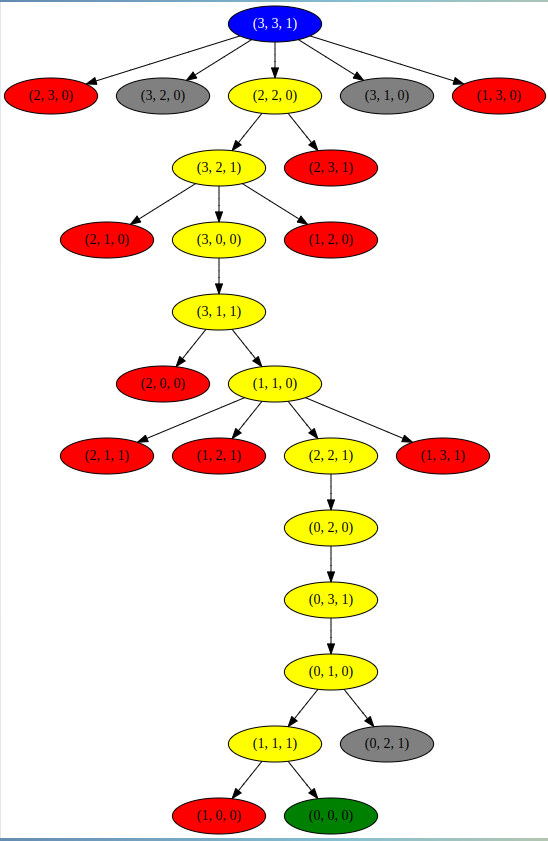
\includegraphics[width = 150mm]{MnC_BFS.png}}
  \caption{Missionaries & Cannibals BFS Solution Tree}
  \label{fig}
\end{figure}
The \texttt{BFS()} function returns \texttt{False} after exploring all possible states without reaching the goal state. If the goal state is encountered, the function returns\texttt {True} within the loop.
\clearpage
\subsection{Search Space Tree}
A search space tree of the possible space was created. The depth of the search space can be controlled by a variable \texttt{max\_depth}
\begin{figure}[h]
  \centerline{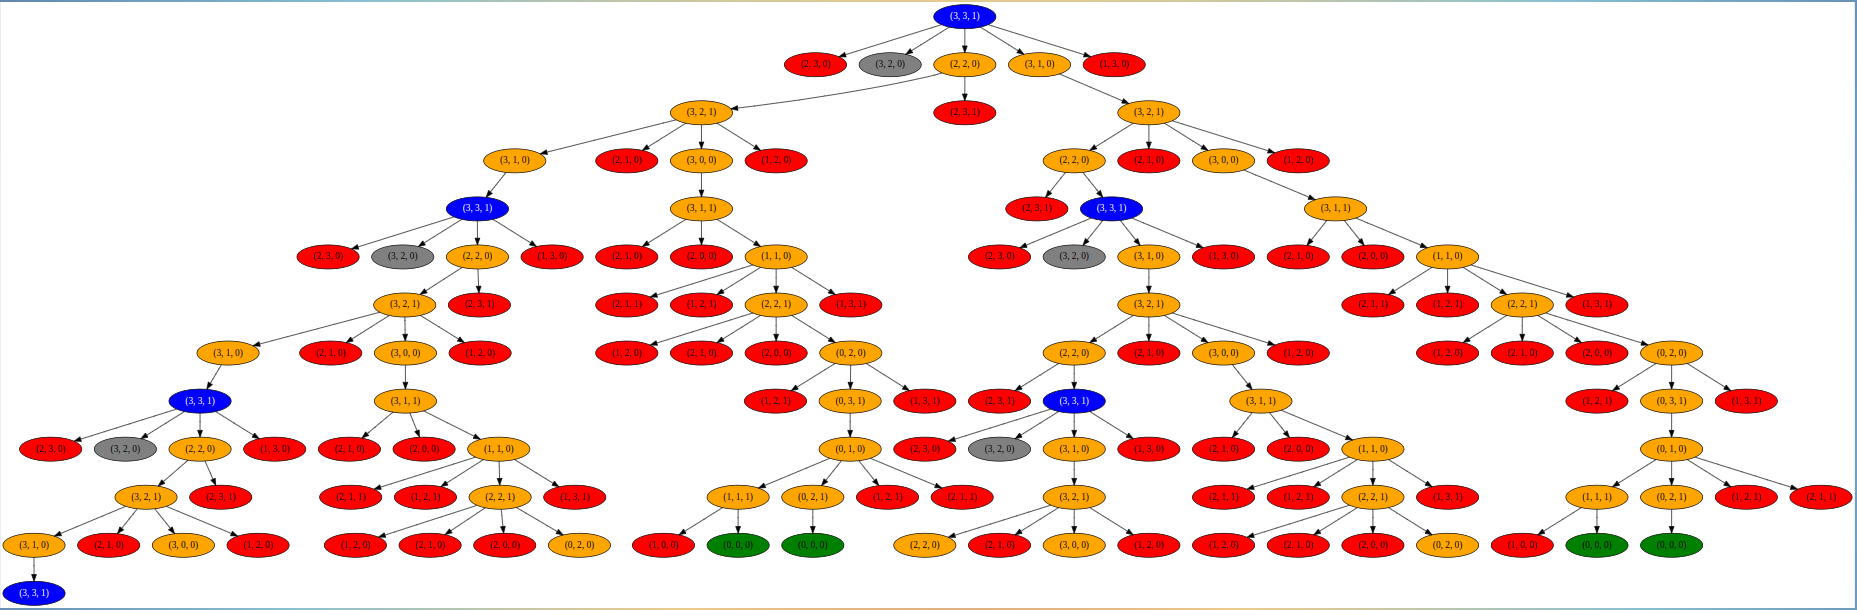
\includegraphics[width = 150mm]{MnC_Space.png}}
  \caption{Missionaries & Cannibals Solution Space Tree}
  \label{fig}
\end{figure}

%%%%%%%%%%%%%%%%%%%%%
\clearpage
%%%%%%%%%%%%%%%%%%%%%
\section{8 Puzzle Problem}
\subsection{Problem Definition}
The 8 Puzzle Problem, also known as the 8-puzzle or sliding puzzle, is a classic puzzle in artificial intelligence and computer science. It involves a 3x3 grid with eight numbered tiles and one empty space. The goal is to rearrange the tiles by sliding them into the empty space, aiming to achieve a specific configuration, usually in ascending order. The puzzle is initiated with a random arrangement of tiles, and the challenge is to find a sequence of moves that transforms this initial state into the desired goal state.

\begin{figure}[h]
  \centerline{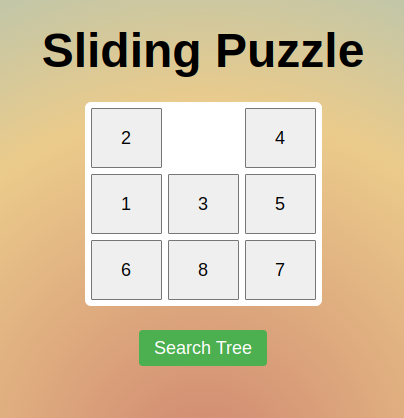
\includegraphics[width = 80mm]{Sliding_Game_demo.png}}
  \caption{Sliding Game Demo}
  \label{fig}
\end{figure}

\begin{figure}[h]
  \centerline{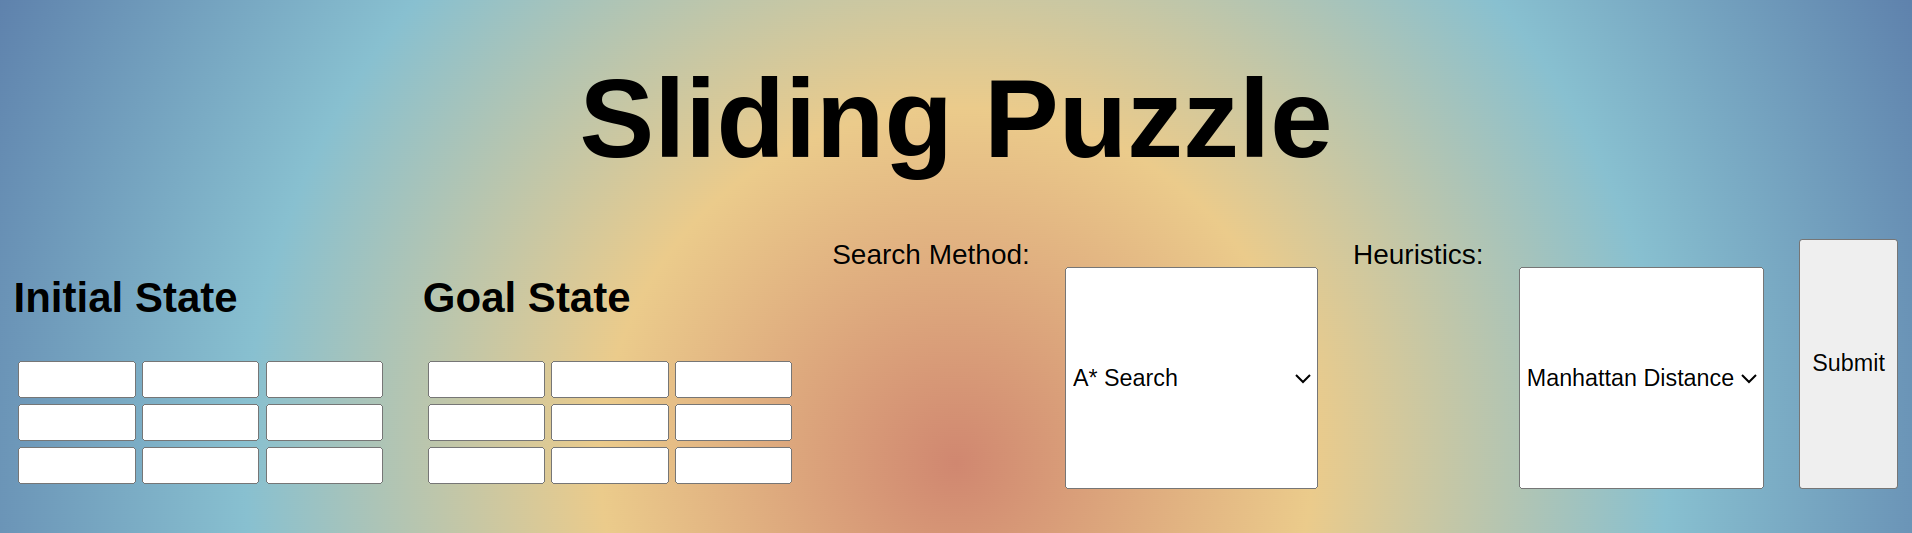
\includegraphics[width = 150mm]{Sliding_Input_demo.png}}
  \caption{8 Puzzle Input Demo}
  \label{fig}
\end{figure}

\textbf{The constraints are as follows:}
\begin{itemize}
    \item The puzzle is played on a 3x3 grid, limiting the number of positions for tiles and the empty space.
    \item At any given time, there can be only one empty space on the grid, which allows for tile movements.
    \item Only tiles adjacent to the empty space can be moved into that space. Diagonal moves are not allowed.
    \item The puzzle has a predetermined goal state that players must aim to achieve. Typically, this is an ordered arrangement of tiles (e.g., sorted in ascending order).
    \item The puzzle must be solvable from a given initial state to the goal state. Not all configurations are solvable, and the solubility of a state is a crucial consideration.
\end{itemize}

\subsection{Search Space Representation}
To represent the search space for the 8 Sliding Puzzle, the code utilizes a
Python class named \texttt{Solver}. The key components of the search space representation are
outlined below:
\begin{minted}[breaklines]{python}
class Solver():
    def __init__(self, state, goal_state, level, parent = None, heuristic_func = "manhattan"):
        self.__state = state
        self.__goal_state = goal_state
        self.__level = level
        self.__heuristic_func = heuristic_func
        self.__heuristic_score = level
        self.__parent = parent
        self.calculate_fitness()
\end{minted}
\begin{itemize}
  \item \texttt{\_\_init\_\_} method initializes the instance with the given parameters.
  \item \texttt{state}: Current state of the puzzle.
  \item \texttt{goal\_state}: The goal state or the target configuration of the puzzle.
  \item \texttt{level}: The depth or level of the state in the search tree.
  \item \texttt{parent}: The parent state from which the current state is derived. (Default is set to \texttt{None} for the initial state)
  \item \texttt{heuristic\_func}: The heuristic function used for estimating the cost.
\end{itemize}

\subsection{Solution via A-Star Search}
\subsubsection*{Manhattan Distance Heuristic}
\begin{itemize}
    \item The solver initializes a priority queue (\texttt{nodes}) and adds the initial state to it.
    \item It then iteratively explores states until the goal state is reached or the maximum number of iterations (\texttt{max\_iter}) is exceeded.
    \item The states are prioritized based on their cost, which is a combination of the current level and the Manhattan Distance heuristic.
    \item If a state is visited before, it is skipped to avoid cycles.
    \item When the goal state is reached, the solver backtracks to reconstruct the solution path and calculates the summary, including the number of steps, nodes visited, and the time taken.
\end{itemize}
\clearpage
\begin{figure}[h]
  \centerline{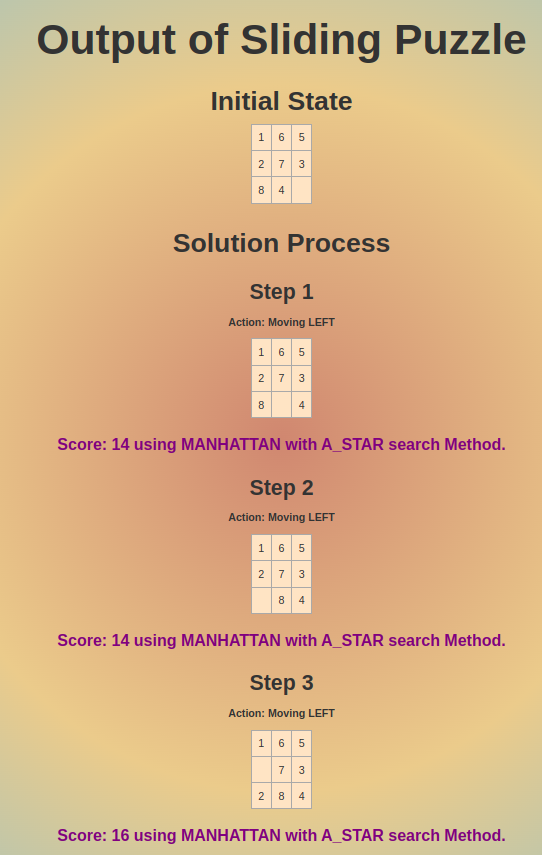
\includegraphics[height = 150mm]{Sliding_Output_M_A_1.png}}
  \caption{8 Puzzle A star Manhattan Demo (beginning)}
  \label{fig}
\end{figure}

\begin{figure}[h]
  \centerline{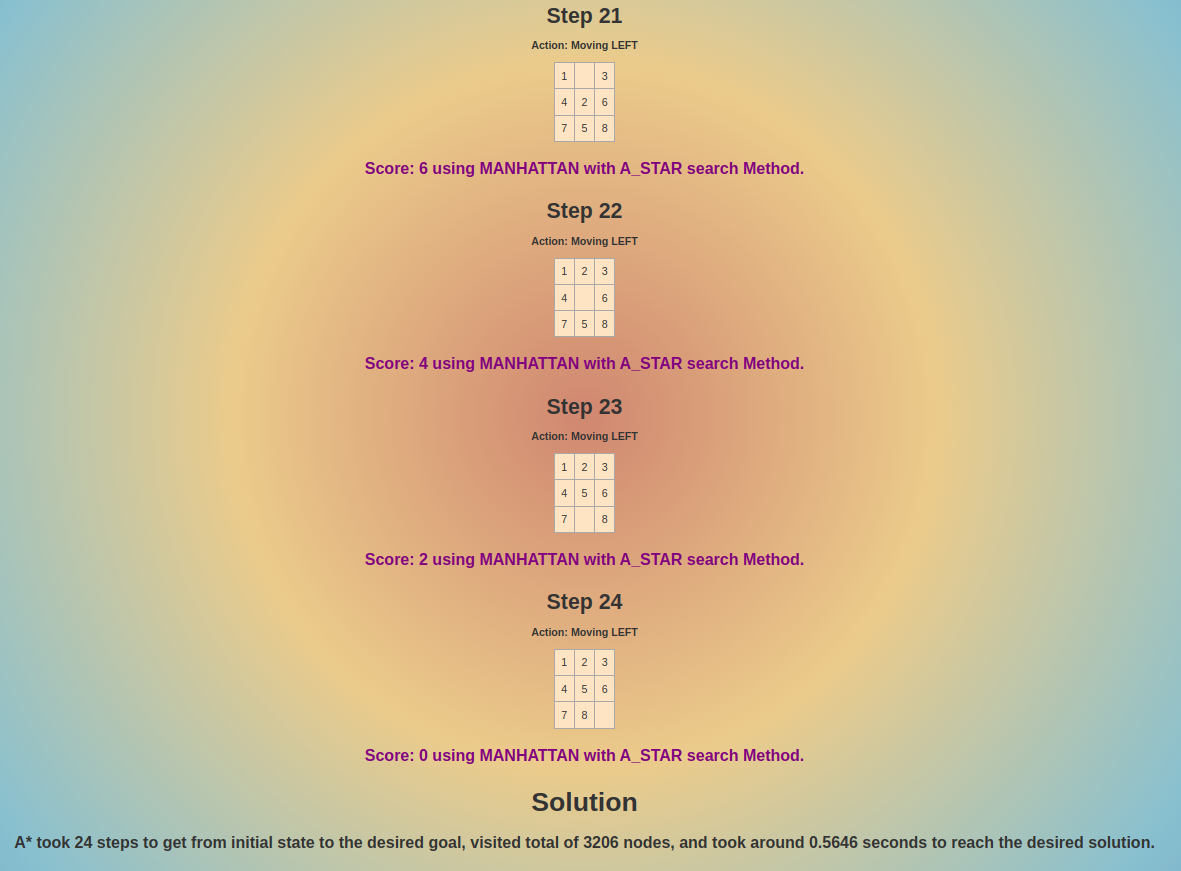
\includegraphics[width = 150mm]{Sliding_Output_M_A_n.png}}
  \caption{8 Puzzle A star Manhattan Demo (beginning)}
  \label{fig}
\end{figure}

\clearpage
\subsubsection*{Tile Moved Heuristic}
\begin{itemize}
    \item The process is similar to the Manhattan Distance heuristic, but the priority of states is determined by the Tiles Moved heuristic.
    \item The Tiles Moved heuristic estimates the cost based on the number of tiles that are out of place in the current state compared to the goal state.
    \item The solver explores states based on their estimated cost using the Tiles Moved heuristic and follows the same process as described for the Manhattan Distance heuristic.
\end{itemize}

\subsection{Solution via BFS}
\subsubsection*{Manhattan Distance Heuristic}
\begin{itemize}
        \item The solver starts by initializing a queue (nodes) and adds the initial state to it.
        \item The BFS algorithm explores states in a breadth-first manner, visiting all neighboring states of the current state before moving to the next level.
        \item The Manhattan Distance heuristic guides the exploration by estimating the cost based on the sum of the Manhattan distances of each tile from its current position to its goal position.
        \item As the BFS explores states, it ensures to avoid revisiting previously explored states (cycles).
        \item Upon reaching the goal state, the solver backtracks to reconstruct the solution path, providing details such as the number of steps taken, nodes visited, and the time elapsed.
\end{itemize}
\subsubsection*{Tile Moved Heuristic}
\begin{itemize}
        \item The BFS algorithm remains consistent, but the heuristic guiding the exploration now changes to Tiles Moved.
        \item Unlike the Manhattan Distance heuristic, which considers the distances of tiles from their goal positions, the Tiles Moved heuristic focuses on the count of tiles that are out of their correct positions.
        \item As with the Manhattan Distance version, BFS explores states based on the estimated cost using the Tiles Moved heuristic.
        \item When the goal state is found, similar backtracking occurs to outline the solution path, along with the associated metrics like steps taken, nodes visited, and execution time.
\end{itemize}

\clearpage
\section{Water Jug Problem}
\subsection{Problem Definition}
The Water Jug Problem involves two water jugs of different capacities and the task of measuring out a specific quantity of water using these jugs. In this specific case, the problem was to use two jugs of 5 liters and 3 liters to measure out 4 liters of water.
\\\\
\begin{figure}[h]
  \centerline{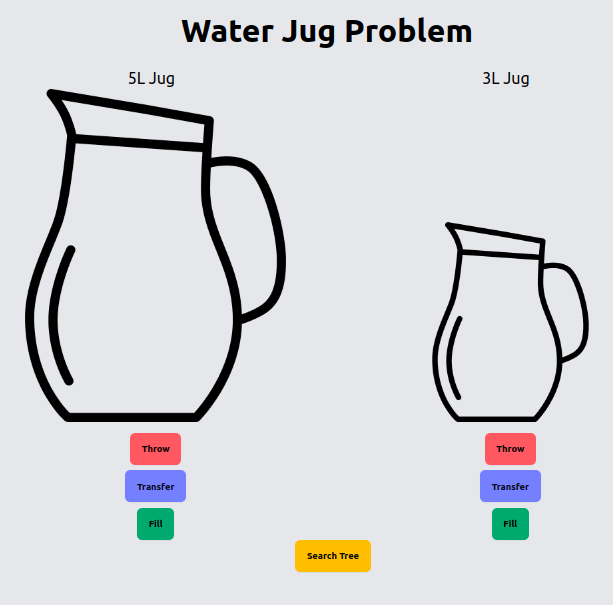
\includegraphics[width = 100mm]{WaterJug_demo.png}}
  \caption{Water Jug Demo}
  \label{fig}
\end{figure}

\textbf{This can be defined as follows:}

\begin{itemize}
    \item \textbf{Jugs:} Two jugs, 5L and 3L capacities.
    \item \textbf{Goal:} Measure 4 liters of water.
    \item \textbf{Initial State:} Both jugs are initially empty (0 liters).
\end{itemize}

\textbf{Operations Allowed:}
\begin{enumerate}
    \item \textbf{Fill Operation:}
    \begin{itemize}
        \item Fill the 5L jug to its full capacity.
        \item Fill the 3L jug to its full capacity.
    \end{itemize}
    \item \textbf{Empty Operation:}
    \begin{itemize}
        \item Empty the water in the 5L jug.
        \item Empty the water in the 3L jug.
    \end{itemize}
    \item \textbf{Transfer Operation:}
    \begin{itemize}
        \item Pour water from the 5L jug to the 3L jug.
        \item Pour water from the 3L jug to the 5L jug.
    \end{itemize}
\end{enumerate}

\textbf{Constraints:}
\begin{itemize}
    \item Jugs cannot hold more water than their capacities.
    \item Goal is achieved when either jug contains exactly 4 liters.
\end{itemize}


\subsection{Solution via DFS}
\begin{figure}[h]
  \centerline{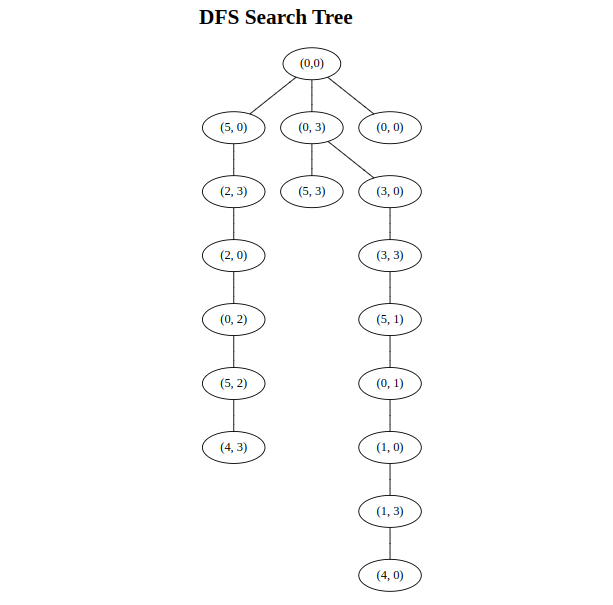
\includegraphics[width = 150mm]{WaterJug_DFS.png}}
  \caption{Water Jug DFS Solution Tree}
  \label{fig}
\end{figure}
\begin{enumerate}
    \item \textbf{Initialization:}
        \begin{itemize}
            \item The DFS tree starts with the initial state, where both jugs are empty \((0,0)\).
            \item The tree is generated in a depth-first manner, exploring as far as possible along each branch before backtracking.
        \end{itemize}
    
    \item \textbf{Exploration:}
        \begin{itemize}
            \item The search space is explored by filling and emptying the jugs and transferring water between them.
            \item Nodes (states) are expanded until the goal state \((4,0)\) is reached or the entire search space is explored.
        \end{itemize}
    
    \item \textbf{Visualization:}
        \begin{itemize}
            \item The DFS tree is visualized using the Pydot library, with nodes representing states and directed edges indicating transitions between states.
        \end{itemize}
    
    \item \textbf{Result:}
        \begin{itemize}
            \item The DFS solution may not be optimal, and the search process heavily depends on the order of exploration. DFS might find a solution faster, but it may not be the shortest path.
        \end{itemize}
\end{enumerate}

\subsection{Solution via BFS}
\begin{figure}[h]
  \centerline{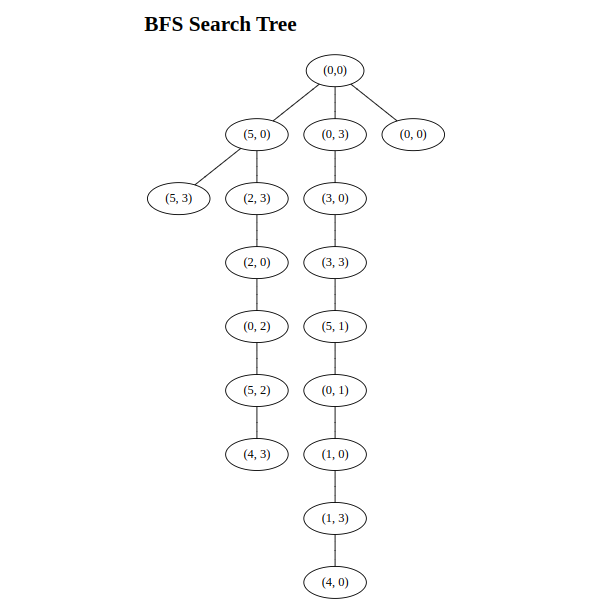
\includegraphics[width = 150mm]{WaterJug_BFS.png}}
  \caption{Water Jug BFS Solution Tree}
  \label{fig}
\end{figure}
\begin{enumerate}
    \item \textbf{Initialization:}
        \begin{itemize}
            \item The BFS tree also starts with the initial state \((0,0)\).
            \item The tree is generated in a breadth-first manner, exploring all nodes at the current depth before moving on to the next level.
        \end{itemize}
    
    \item \textbf{Exploration:}
        \begin{itemize}
            \item Similar to DFS, BFS explores the search space by applying operations to the states.
            \item BFS ensures optimality by exploring all states at a given depth before moving deeper into the search space.
        \end{itemize}
    
    \item \textbf{Visualization:}
        \begin{itemize}
            \item The BFS tree is visualized using Pydot, with nodes and edges representing states and transitions, respectively.
        \end{itemize}
    
    \item \textbf{Result:}
        \begin{itemize}
            \item BFS is guaranteed to find the shortest path to the goal state. It explores the search space level by level, ensuring that the first solution found is the optimal one.
        \end{itemize}
\end{enumerate}


\section{Technologies/Libraries Used}


The implementation of the Water Jug, Missionaries and Cannibals, Sliding Puzzle Problem, and its solution strategies involves the utilization of several technologies and libraries. These tools contribute to the development, visualization, and analysis of the search space and solution paths.

\subsection*{Python Programming Language}

Python serves as the primary programming language for developing the algorithms and logic behind the Water Jug Problem. Its simplicity, readability, and extensive standard library make it well-suited for implementing complex problem-solving algorithms and data structures.

\subsection*{Flask}

Flask, a web framework for Python, is employed to create a simple web application that visualizes the search trees generated during the solution process. It facilitates the rendering of HTML templates and serves as the backbone for hosting the application.

\subsection*{Pydot}

Pydot is a Python interface to Graphviz, a graph visualization tool. Pydot enables the creation of visual representations of the search trees generated by BFS and DFS. The graphs illustrate the exploration process and solution paths, providing a clear visual understanding of the algorithmic steps.

\subsection*{Queue and PriorityQueue (from Python's queue Module)}

The `Queue` and `PriorityQueue` classes from the Python `queue` module are used to manage the states during BFS and A* search algorithms, respectively. These data structures streamline the exploration of the search space by providing a convenient way to maintain and process the states in a first-in-first-out (FIFO) or priority order.

\subsection*{Numpy}

Numpy, a powerful numerical computing library in Python, is employed for handling matrix operations and representing the states of the Water Jug Problem. Its array manipulation capabilities simplify the implementation of the puzzle's initial and goal states, as well as the transition between states.

\subsection*{Time Module}

The `time` module in Python is utilized to measure the execution time of the search algorithms. It helps in analyzing the efficiency of the implemented strategies and provides insights into the computational aspects of solving the Water Jug Problem.

\subsection*{HTML and CSS}

HTML and CSS are used for creating the user interface of the web application. HTML templates structure the content, while CSS styles enhance the visual presentation, ensuring a user-friendly and aesthetically pleasing interface.

\subsection*{Additional Python Modules}

\begin{itemize}
    \item \textbf{os:} The `os` module is used for interacting with the operating system. It may be utilized for tasks such as file operations and environment management within the project.
    
    \item \textbf{emoji:} The `emoji` module adds support for Emoji glyphs. While not directly involved in the core logic, it can be used to enhance the visual aspects of the application.
    
    \item \textbf{random:} The `random` module is used for generating pseudo-random numbers. It can be applied for scenarios involving randomness or shuffling within the project.
    
    \item \textbf{collections:} The `collections` module is used for deque operations. The `deque` class provides a double-ended queue, which is beneficial for efficiently implementing certain algorithms.
\end{itemize}

These technologies and libraries, along with the additional Python modules, collectively contribute to the successful implementation, visualization, and analysis of the Water Jug Problem and its solution strategies within the project.


\section{Conclusion}

\subsection{Insights}

The exploration of various search methods for the Missionary and Cannibal Problem, 8 Puzzle Problem, and Water Jug Problem has provided valuable insights into the application of algorithmic techniques to solve diverse challenges. The insights gained from each problem are summarized below:

\subsubsection{Missionary and Cannibal Problem}
The implementation of Breadth-First Search (BFS) and Depth-First Search (DFS) has demonstrated the effectiveness of these methods in finding solutions to constrained problems like the Missionary and Cannibal Problem. BFS ensures optimality by exploring all possible states at each level, while DFS efficiently explores deeper states first, possibly finding a solution faster.

\subsubsection{8 Puzzle Problem}
The exploration of the A* search algorithm with two different heuristics, namely Manhattan Distance and Tiles Moved, has shed light on the impact of heuristic choices on solution efficiency. The Manhattan Distance heuristic prioritizes states based on their spatial proximity to the goal, while Tiles Moved counts the number of misplaced tiles. The choice of heuristic significantly influences the speed and optimality of the solution path.

\subsubsection{Water Jug Problem}
The Water Jug Problem has provided insights into the application of search algorithms in a problem domain involving state transitions and constraints. Both BFS and DFS have proven effective in finding solutions to the Water Jug Problem. The visualization of the search space has enhanced the understanding of how these algorithms explore and navigate the problem space.

\subsection{Further Work}

While the implemented search methods have shown success in solving the specified problems, there exist opportunities for further research and improvement:

\subsubsection{Enhanced Heuristics}
For problems like the 8 Puzzle, exploring more sophisticated heuristics may lead to improvements in solution efficiency. Experimenting with novel heuristic functions could enhance the A* algorithm's ability to guide the search towards optimal paths.

\subsubsection{Parallelization and Optimization}
Investigating parallelization techniques and algorithmic optimizations could be beneficial, especially when dealing with larger problem instances. This includes exploring parallel versions of search algorithms to leverage modern multi-core processors and optimizing data structures for more efficient state exploration.

\subsubsection{Real-world Applications}
Applying the learned methodologies to real-world problems with similar structures could provide practical insights. Extending the techniques developed for the discussed problems to domains such as resource optimization, scheduling, or network routing may uncover novel applications.

\subsubsection{User Interaction and Experience}
Improving the user interface and interaction aspects of the presented solutions, especially in the web-based visualizations, can enhance the educational and explanatory value of the project. This includes incorporating interactive features, additional visual cues, and user-friendly controls.

In conclusion, the exploration of these search methods opens avenues for continued research and application, paving the way for advancements in both theoretical understanding and practical problem-solving strategies.

\clearpage
\thispagestyle{empty}
\bibliographystyle{IEEEtran}
\bibliography{references}

\end{document}

